\subsection{Firefighter Agent Crew}

The Firefighter Agent Crew operates within a structured \textbf{sequential process} to ensure effective and coordinated response to fire emergencies. Each task is assigned to a specific agent with well-defined responsibilities, as detailed below:

\begin{enumerate}
    \item \textbf{Receive Report:} The \textit{Fire Chief} receives a fire assessment from the Emergency Service Operator. This serves as the starting point of the process, containing critical information such as the location and severity of the fire.
    \item \textbf{Allocate Firefighting Resources:} The \textit{Equipment Technician} determines if there exact resources required to combat the fire in question.
	\item \textbf{Deploy Fire Combatants:} The \textit{Fire Combatants} are deployed to the place of the fire, reporting an estimation of the time of arrival and a list of the fire fighting activities that will have to be performed.
	\item \textbf{Report Firefighting Response:} The \textit{Fire Chief} reports back a comprehensive summary of the firefighting activities.
\end{enumerate}

\paragraph{Task Dependencies}
The sequential process relies on strict task dependencies to maintain an organized workflow:
\begin{itemize}
    \item \textit{Allocate Firefighting Resources} depends on the completion of \textit{Receive Report}.
    \item \textit{Deploy Fire Combatants} depends on the completion of \textit{Deploy Fire Combatants}.
    \item \textit{Report Firefighting Response} depends on the completion of \textit{Deploy Fire Combatants}.
\end{itemize}

The visual representation in Figure~\ref{fig:firefighter_flow} highlights these dependencies and assigns colors to denote the responsible agents.

\begin{figure}[ht!]
	\centering
	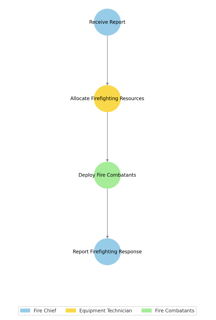
\includegraphics[height=0.59\textheight]{figures/Firefighter_Crew_Flow.png}
	\caption{Sequential Process Flow of the Firefighter Crew with Agent Responsibilities}
	\label{fig:firefighter_flow}
\end{figure}

